%%%%%%%%%%%%%%%%%%%%%%%%%%%%%%%%%%%%%%%%%%%%%%%%%%%%%%%%%%%%%%%%%%%%%%%%%%%%%%%%
%2345678901234567890123456789012345678901234567890123456789012345678901234567890
%        1         2         3         4         5         6         7         8

\documentclass[letterpaper, 10 pt, conference]{ieeeconf}  % Comment this line out if you need a4paper
%\documentclass[a4paper, 10pt, conference]{ieeeconf}      % Use this line for a4 paper

\IEEEoverridecommandlockouts                              % This command is only needed if 
                                                          % you want to use the \thanks command

\overrideIEEEmargins                                      % Needed to meet printer requirements.

% See the \addtolength command later in the file to balance the column lengths
% on the last page of the document

% The following packages can be found on http:\\www.ctan.org
\usepackage{graphics} % for pdf, bitmapped graphics files
\usepackage{epsfig} % for postscript graphics files
\usepackage{mathptmx} % assumes new font selection scheme installed
\usepackage{times} % assumes new font selection scheme installed
\usepackage{amsmath} % assumes amsmath package installed
\usepackage{amssymb}  % assumes amsmath package installed
% \usepackage{comment}
% \usepackage{algorithm,algpseudocode}
% \usepackage{resizegather}
% \usepackage{flexisym}
\usepackage{dblfloatfix}    % To enable figures at the bottom of pag
\usepackage{subcaption}
\usepackage{mathtools}
% \usepackage[square,numbers]{natbib}

% TODO: french letter in name
% \usepackage{inputenc} 

\title{\Large \bf Social RL: Socially Compliant Navigation in Crowds
with Deep Reinforcement Learning}

\author{% <-this % stops a space
\thanks{This work was supported by [?]}% <-this % stops a space
% \thanks{$^{1}$L is with, 
% {\tt\small b.d.researcher@ieee.org}}%
% \thanks{$^{*}$Equal contribution}       
\thanks{Visual Intelligence for Transportation Laboratory, Ecole Polytechnique Federale de Lausanne (EPFL)
, CH-1015 Lausanne,
        {\tt\small \{ \}@epfl.ch}}%
}

\begin{document}

\bstctlcite{IEEEexample:BSTcontrol}

\maketitle
\thispagestyle{empty}
\pagestyle{empty}

\pdfminorversion=4  
%%%%%%%%%%%%%%%%%%%%%%%%%%%%%%%%%%%%%%%%%%%%%%%%%%%%%%%%%%%%%%%%%%%%%%%%%%%%%%%%
\begin{abstract}
[TODO]
\vspace{3cm}

\end{abstract}


%%%%%%%%%%%%%%%%%%%%%%%%%%%%%%%%%%%%%%%%%%%%%%%%%%%%%%%%%%%%%%%%%%%%%%%%%%%%%%%%
\section{INTRODUCTION} \label{sec:intro}

With the rapid growth of machine intelligence, robots are envisioned to expand habitats from isolated environments to social spaces that are shared with humans and other embodied agents. Traditional approaches for robot navigation often view the moving agents nearby as static obstacles \cite{fox_dynamic_1997} or react to them through a one-step lookahead \cite{berg_reciprocal_2008}, resulting in short-sighted and unsafe / unnatural behaviors. In order to navigate through a crowd in a socially compliant manner, robots need the ability to understand the behaviors of the others while making its movement decision. 

Navigation with social etiquettes is, however, a very challenging task. As communications among agents (e.g. robots, pedestrians, bikers) are not widely available, robots need to by itself perceive and anticipate the evolution of the crowd, which can involve complex interactions. Research works in trajectory prediction have proposed several hand-crafted or data-driven methods to model the agent-agent interactions \cite{helbing_social_1995,alahi_social_2016,vemula_social_2017,gupta_social_2018}. However, even assuming we have a good predictive model, how to integrate the interaction knowledge into the decision-making process remains another challenge. 

Earlier works split the prediction and planning into two separate steps, attempting to identify a safe trajectory distant from the forecasted regions of the other agents \cite{bennewitz_learning_2005,aoude_probabilistically_2013}. However, the probabilistic untraversable regions in the next steps can be very large in a crowded scene, causing the freezing robot problem \cite{trautman_unfreezing_2010}. To cope with it, a large number of works have been focused on the joint obstacle avoidance methods that plan the paths of all the interactive decision-makers simultaneously, in hope to make navigation rooms for each other cooperatively \cite{trautman_unfreezing_2010}. Though conceptually desirable, these methods often suffer from the stochasticity of the neighbors' behaviors as well as the computational costs in practice. 

As an alternative, the reinforcement learning framework has been used to train a computationally efficient policy that implicitly encodes the interactions and cooperations among agents. While great progress has been made in recent works \cite{chen_decentralized_2016,chen_socially_2017,long_towards_2017,everett_motion_2018}, existing models are limited in two aspects. i) The joint impact of the neighboring agents on the navigator is usually modeled by a simplified aggregation of the pairwise interactions, such as a Maximin operator or LSTM, which can hurt the scalability of the encoded cooperation to dense crowds severely. ii) They are focused on the one-way interactions from the crowd to the navigator but omit the interactions within the crowd that essentially shape the hidden state of each interactive neighbor and eventually affect the navigator. These limitations may degrade the performance of cooperative planning-based reasoning in complex and crowded scenes. 

\begin{figure} [t]
  \captionsetup{font=small}
  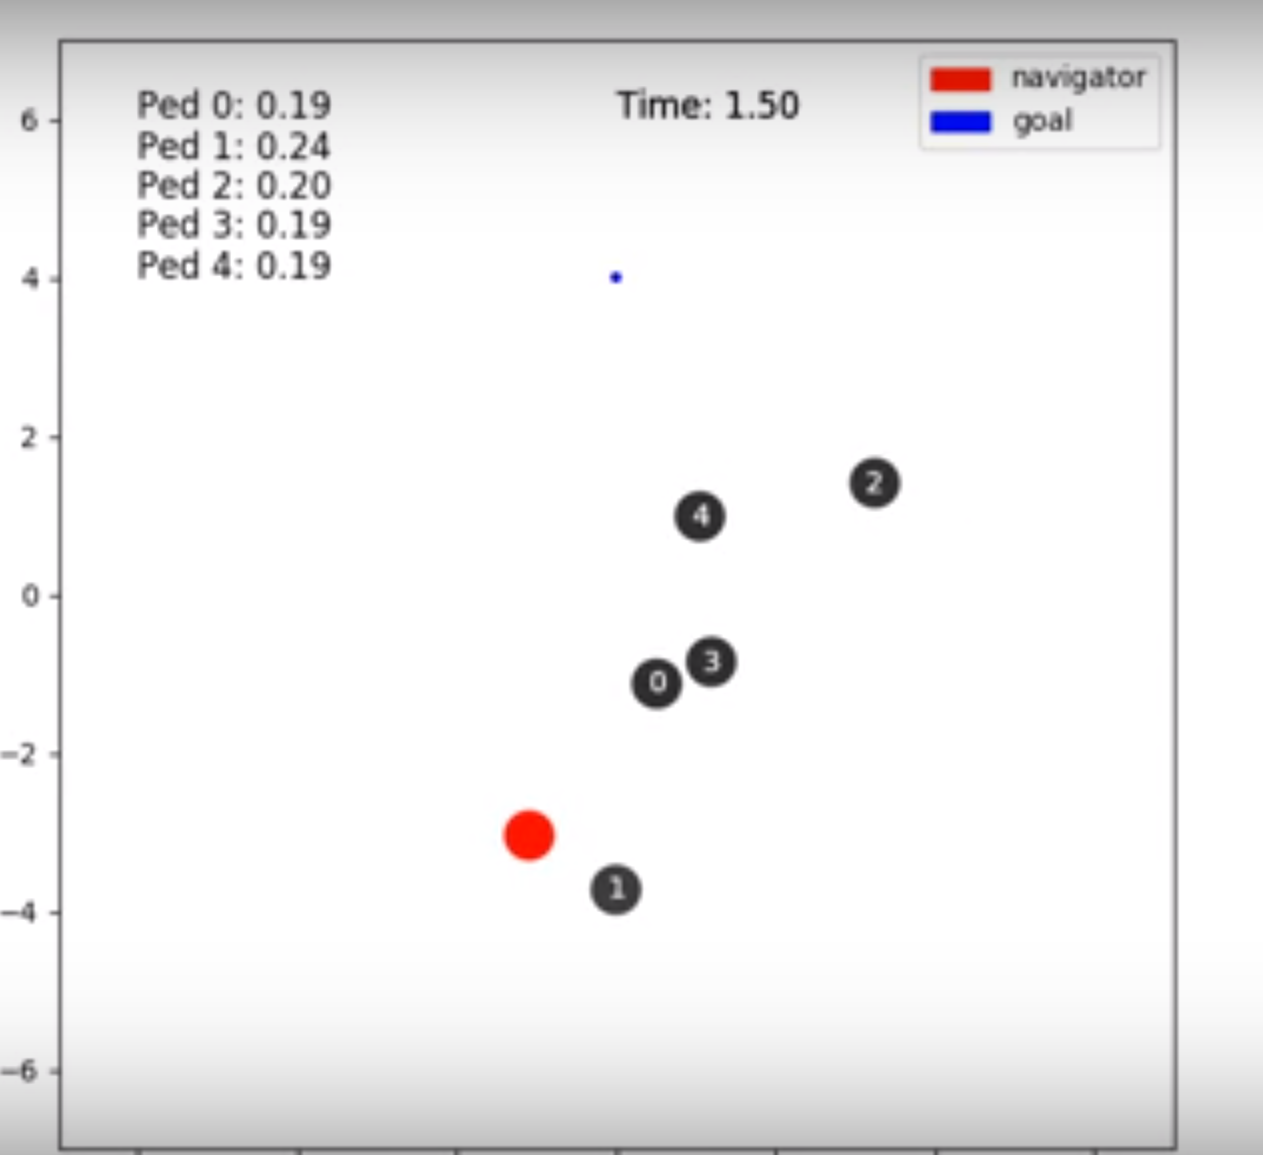
\includegraphics[width=0.2\textwidth]{figures/overview}
  \caption{TODO: Illustration of the socially compliant navigation in a crowded scene.}
  \label{fig:overview}
\end{figure}

In this work, we propose a novel pooling module for the reinforcement learning method, aiming to learn a socially compliant navigation policy in complex scenes. Inspired by \cite{alahi_social_2016,gupta_social_2018,vemula_social_2017}, we first extract the features of the pairwise social interaction between the navigator and each of its neighbors and subsequently use the soft attention to learn the importance of these interactions. In addition, we encode the impact of intra-interaction on each agent by a local occupancy map. Based on a weighted aggregation, our model can naturally take an unlimited number of neighboring agents into account and provide a good understanding of the crowd in the form of value estimation, from which a cooperative action command can be derived at each step. An extensive set of experiments shows that our approach can effectively learn to perceive the behaviors of the other agents and navigate through them in a socially compliant manner, outperforming the state-of-the-art methods. 

\section{BACKGROUND} \label{sec:background} 

\subsection{Related Work}

Existing works on cooperative navigation have been extensively focused on the joint obstacle avoidance. The reactive methods such as RVO \cite{berg_reciprocal_2008} and ORCA \cite{van_den_berg_reciprocal_2011} seek the joint collision-free velocities under the reciprocal assumption, which have been successfully applied to the distributed multi-agent systems. The Interacting Gaussian Process (IGP) method models the trajectory of each agent as an individual Gaussian Process and introduces an interaction potential to couple the individual GP in a principled statistical way. The main challenge for these model is that the hand-crafted functions cannot generalize well to the human-like cooperations in various scenarios. 

Another line of works uses the imitation learning approach to program a socially compliant policy from the demonstrations of good cooperative behaviors. \cite{tai_socially_2017} and \cite{long_deep-learned_2017} developed policies that map raw depth images and lidar measurements to actions respectively by directly mimicking the demonstrations. Beyond behavioral cloning, \cite{roy_feature-based_2013, kretzschmar_socially_2016, pfeiffer_predicting_2016} learn the underlying cooperation features from the pedestrians data by means of the maximum entropy learning inverse reinforcement learning method. The learning outcomes in these works often highly depend on the scale and quality of demonstrations, which is not only resources consuming but also constrained by an upper bound from the demonstrator. In our work, we adopt the imitation learning approach to warm start our model training and subsequently refine it with reinforcement learning. 

Deep reinforcement learning has been intensively studied in the recent years and applied to various fields since \cite{mnih_human-level_2015} successfully stabilized it for mastering games from train-and-error experiences. With respect to the robot navigation, \cite{tai_virtual--real_2017,long_towards_2017} use the deep reinforcement learning approach to train sensorimotor policies in static and dynamic environments, while \cite{chen_decentralized_2016,chen_socially_2017,everett_motion_2018} develop social policies with the agent-level state information. Specifically, \cite{chen_decentralized_2016} adapts their formulation from the two-agent to the multi-agent cases through a Maximin operation that picks up the best action against the worst-case value rather than the joint value of the crowd. As an extension, \cite{everett_motion_2018} use the LSTM to aggregate the state of each neighbor sequentially in a reverse order of the distance to the navigator. In contrast to these simplifications, we propose a novel neural network model to capture the joint impact of the crowd with fine-grained information. 

A variety of deep neural networks have been proposed in recent years for modeling the human-human interactions and demonstrated competitive results\cite{becker_evaluation_2018}. One of the inspiring attempts is the Social LSTM, which models each individual by an LSTM and couple the states of agents within in a neighborhood through a social pooling module \cite{alahi_social_2016}. The pooling module is later extended to several structures for improved the attention, cooperation as well as computational efficiency \cite{fernando_soft_2017, gupta_social_2018}. Another set of works models the social interactions through spatio-temporal graphs, where attention is also introduced to learn the relative importance of each neighboring agent \cite{vemula_social_2017}. Our work built upon these models designs a special pooling module to encode cooperative behaviors for the socially compliant navigation. 

Attention \cite{vaswani_attention_2017}
[TODO?]

\subsection{Problem Formulation}

Consider a navigation task that a robot moves to a goal destination through a crowd of pedestrians $\{1,2,\dots,n\}$. It can be formulated as a decision making problem through a sequence of observations, action, and reward triplets\cite{chen_decentralized_2016,chen_socially_2017,everett_motion_2018}. Let $\bold{s}_t $, $\tilde{\bold{s}}_t = [\tilde{\bold{s}}_t^1, \tilde{\bold{s}}_t^2, \dots, \tilde{\bold{s}}_t^n]$ denote the state of the robot and the pedestrians at time $t$ respectively. Specifically, the full state of the robot is defined as $ \bold{s} = [\bold{p}, \bold{v}, r, \theta, \bold{p_g}, v_{pref}]$ and the observable state of a pedestrian is defined as $ \tilde{\bold{s}}_i = [\bold{p}, \bold{v}, r]$, where $\bold{p}=[p_x,p_y]$ and $\bold{v}=[v_x,v_y]$ are the vectors of location and velocity in the $2D$ plane, $r$ is the radius. We assume that the robot is aware of its unobservable state including the heading angle $\theta$, goal position $\bold{p_g}$ and preferred speed $v_{pref}$ and that the robot velocity can be achieved by the action command $\bold{a}_t$ immediately, $\bold{v}_t = \bold{a}_t$. The joint state for the robot navigation at time $t$ is defined as $\bold{s}_t^{jn} = [\bold{s}_t, \tilde{\bold{s}}_t]$. 

The desired navigation policy, $\pi : \bold{s}_t^{jn} \mapsto \bold{a}_t$, is to maximize the objective function without violating the constraints:
\begin{subequations} \label{eq:optimization}
\begin{align}
& \underset{\pi(\bold{s}^{jn})}{\text{argmax}}
& & \mathbb{E}[\sum_{t=0}^T R_t | \bold{s}_0^{jn}, \bold{p}_g, \pi] \label{eq:obj} \\
& \text{subject to} 
& & \bold{p}_T = \bold{p}_g \label{eq:goal} \\
&&& \bold{p}_{t+\Delta t} = \bold{p}_{t} + \Delta t \pi(\bold{s}_{t}^{jn}) \label{eq:kinematics} ~ & t = 0, \Delta t, \dots, T \\
&&& \left\Vert \bold{p}_t - \tilde{\bold{p}}_t^i \right\Vert >= r + \tilde{r}^i & i = 1, 2, \dots, n \label{eq:safety}
\end{align}
\end{subequations}
where (\ref{eq:obj}) is the expected total reward that the robot can obtain in the navigation task, (\ref{eq:goal}) is the goal constraint, (\ref{eq:kinematics}) is the kinematics of the robot, (\ref{eq:safety}) is the safety constraint, $T$ is the time when reaching the goal, and $\Delta t$ is the time step interval. 

The reward function is defined to penalize the collision and uncomfortable distances and award the task accomplishment, 
\begin{equation}
    R_t(\bold{s}_t^{jn},\bold{a}_t)= 
\begin{dcases}
    -1 & \text{if} ~~ d_t < 0 \\
    -0.25 + d_t & \text{else if} ~~ d_t < 0.2 \\
    1 & \text{else if} ~~ \bold{p}_t=\bold{p}_g \\
    0 & \text{otherwise} 
\end{dcases}
\end{equation}
where $d_t$ is the minimum seperation distance between the robot and the pedestrians during the time period $[t-\Delta t,t]$. 

The problem (\ref{eq:optimization}) can be tackled by a reinforcement learning method that seeks a optimal policy 
\begin{equation} \label{eq:RL}
\begin{split}
\pi^{*}(\bold{s}_t^{jn}) = & \underset{\bold{a}_t}{\text{argmax}} ~ R(\bold{s}_t^{jn},\bold{a}_t) + \\
& \gamma^{\Delta t \cdot v_{pref}} \int_{\bold{s}_{t+\Delta t}^{jn}} P(\bold{s}_t^{jn},\bold{a_t},\bold{s}_{t+\Delta t}^{jn}) V^*(\bold{s}_{t+\Delta t}^{jn}) d\bold{s}_{t+\Delta t}^{jn}
\end{split}
\end{equation}
where $\gamma \in [0,1)$ is a discount factor, $P(\bold{s}_t^{jn},\bold{a_t},\bold{s}_{t+\Delta t}^{jn}) $ is the transition probability from time $t$ to time $t+\Delta t$, during which the robot takes the action $\bold{a_t}$. The state transition probability can be viewed as a trajectory prediction model for a short period of time. 

\begin{figure} [t]
  \captionsetup{font=small}
  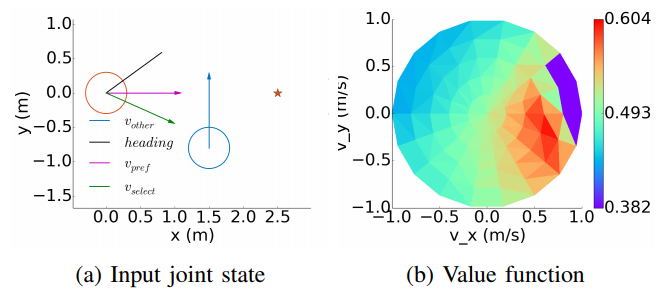
\includegraphics[width=0.5\textwidth]{figures/vf} 
  \caption{TODO: Value function estimation for a navigation task in a densely popullated crowd.}
  \label{fig:overview}
\end{figure}

The optimal value function $V^*$ is an estimate of the expected total reward from time $t$ till the end under the optimal policy $\pi^*$: 
\begin{equation}
V^*(\bold{s}_t^{jn}) = \sum_{t}^T \gamma^{t \cdot v_{pref}} R_t(\bold{s}_t^{jn},\pi^*(\bold{s}_t^{jn}))
\end{equation}
A key challenge for solving the problem (\ref{eq:RL}) is to design an expressive model that can accurately approximate the optimal value function $V^{*}$ encoding the socially cooperative path planning among agents. Previous work on this track involves some simplifications on the group interactions, which weakenes the accuracy of value estimation for a densely populated scene. The goal of this work is to develop an improved social pooling module integrated into the framework for learning a social compliant policy. 

\section{[TODO]APPROACH} \label{sec:approach} 
Two levels of motivation: we use MLP for planning and the input is navigator's state and other pedestrians' information. But since the number of peds varies and the network takes fixed size input. [GA3C-CADRL] proposed to solve the problem by using LSTM and feeds the sorted pedestrian's state in the decreasing order of the distance to the ped. But the distance doesn't necessarily mean the importance of pedestrian. A better way is for agent to reason the relation pairwise with each pedestrian, so it knows which pedestrian he should attend to. When reason other agent's behavior, it's always better to  

The following presents our problem to reason multiagent collision avoidance problem. The whole model consists of three modules, and from low-level to high-level they are ped-ped interaction module, attention module and navigator planning module. The first two modules are specifically designed to better reason pedestrians' future behavior and encode the information of varying number of pedestrians.

\begin{figure}[thpb]
  \centering
    \framebox{\includegraphics[scale=0.1]{figures/model.png}}
  %\includegraphics[scale=1.0]{figurefile}
  \caption{Model Architecture. (Description)}
  \label{figurelabel}
\end{figure}

\subsection{Parameterization}
[TODO]

\subsection{Ped-ped Interaction Modeling}
(describe why the occupancy map is introduced)
Since predicting pedestrians' action without jointly considering the navigator's action usually leads to freezing robot problem. So in this module, both the information of pedestrian, its surrounding environment and navigator's state are taken as input. We use multilayer perceptron to reason that pedestrian's future action give the observation of other agents. And this learned information can be further used for navigator's action planning. Since the number of pedestrians is varying and the neural network takes fixed size tensor input. One way to handling the varying number agents is to use LSTM model or attention model, but then the computation will be $O(n^2)$, which is not very efficient. So here we represent the knowledge of nearby pedestrian's states in an local occupancy map. The local occupancy map is centered at that pedestrian and aligned with its velocity. Each cell of the grid is represented as the average velocity of pedestrians who occupy that cell. 

\subsection{Attention Mechanism}
(how the attention model works and formulation)

\section{RESULTS}

\subsection{Implementation Details}
In this work, we choose ORCA [] as the policy for pedestrians. ORCA is a reaction-based collision avoidance algorithm and it can guarantee local collision avoidance. And we integrate the public available https://github.com/snape/RVO2 into our framework. To better simulate the real world distribution of pedestrian behaviors and avoid the identical behaviors of pedestrians, the parameters of ORCA for each pedestrians is sampled from certain distribution. So both radius, preferred speed varies from pedestrian to pedestrian.

The training and testing cases are all crossing scenarios, where agents are positioned on a circle of certain radius and their goals are on the opposite side of circle. Perturbation is added to the x and y coordinates of pedestrians to simulate varying time differences when two agents meet. In test, there are 500 randomly generated test cases.

Compared to multiagent training, in non-reciprocal setting, it's harder to evaluate the policy since in the most extreme case, if one agent goes straight to his goal without slowing down, then all the agents on his way can simply give their paths to him, which results in the shortest time for him to reach goal. But for the other agents, their behaviors will be influenced by that agent. Thus, we first conducted experiments on non-cooperative setting, where the navigator is invisible and it has to learn how to navigate seamlessly. We did the same experiments with the navigator visible and added another metrics to measure the cooperativeness of the navigator. 

(timing requirements)

\subsection{Methods Evaluated}
We considered five approaches: one reaction-based, five learning based reinforcement learning algorithms but with different state learning models.

\begin{itemize}

\item ORCA
\item CADRL
\item LSTM-RL
\item SRL
\item SARL
\item OM-SARL

\end{itemize}

\subsection{Measurement Metrics}

\begin{itemize}

\item Success rate.
\item Collision rate.
\item Extra time for navigator to reach goal(ET-NAV).
\item Average extra time for pedestrians to reach goal(ET-AVG-PED).
\item Extra time for last pedestrian to reach its goal(ET-LAST-PED).
\item Average times of being too close to other pedestrians per second.

\end{itemize}

\subsection{Performance Comparison on Non-cooperative Agents}

\begin{table}[h]
\caption{Comparison of all the methods}
\label{table_example}
\begin{center}
\begin{tabular}{|c||c|c|c|}
\hline
Methods & Success rate & Collision rate & ET-NAV\\
\hline
ORCA &  &  &\\
\hline
CADRL &  &  &\\
\hline
LSTM-RL &  &  &\\
\hline
SRL &  &  &\\
\hline
SARL &  &  &\\
\hline
OM-SARL &  &  &\\
\hline
\end{tabular}
\end{center}
\end{table}

\subsection{Performance Comparison on Cooperative Agents}

\begin{table}[h]
\caption{Comparison of all the methods}
\label{table_example}
\begin{center}
\begin{tabular}{|c||c|c|c|c|c|}
\hline
Methods & Success rate & Collision rate & ET-NAV & ET-AVG-PED & Too-close/s\\
\hline
ORCA &  &  & & & \\
\hline
CADRL &  &  & &  &\\
\hline
LSTM-RL &  &  & & &\\
\hline
SRL &  &  & & &\\
\hline
SARL &  & & & &\\
\hline
OM-SARL  &  & & & &\\
\hline
\end{tabular}
\end{center}
\end{table}

\subsection{Hardware Experiment}

\section{CONCLUSION}

% Formulation, 

% \section{RESULTS} \label{sec:results} 

% Simulation experiments, 

% Real-world experiments, and video. 

% \section{CONCLUSION} \label{sec:conclusion} 

% In this paper, 

% \subsection{System Structure}

\addtolength{\textheight}{-10cm}   % This command serves to balance the column lengths
                                  % on the last page of the document manually. It shortens
                                  % the textheight of the last page by a suitable amount.
                                  % This command does not take effect until the next page
                                  % so it should come on the page before the last. Make
                                  % sure that you do not shorten the textheight too much.

\section*{ACKNOWLEDGMENT}

% We would like to thank ... 

\bibliographystyle{IEEEtran}
\bibliography{vita-social-nav}

% \begin{thebibliography}{99}

% \end{thebibliography}

\end{document}


% @IEEEtranBSTCTL{IEEEexample:BSTcontrol,
%   CTLuse_url = "no",
%   CTLuse_article_number = "yes",
%   CTLuse_paper = "yes",
%   CTLuse_forced_etal = "yes",
%   CTLmax_names_forced_etal = "4",
%   CTLnames_show_etal = "1",
%   CTLuse_alt_spacing = "yes",
%   CTLalt_stretch_factor = "4",
%   CTLdash_repeated_names = "yes",
%   CTLname_latex_cmd = ""
% }